%-----------------------------------------------------------------------------------------------------------
% Everything before \begin{document} and
% \end{document} is called Preamble. The Preamble
% sets up your document. The preamble typically specifies
%   the document class
%   languages
%   imports packages by using \usepackage{package_name} command
%-----------------------------------------------------------------------------------------------------------

%-----------------------------------------------------------------------------------------------------------
% Note: A latex command consist of a backslash, command name, argument (with {}) #
% and optional arguments (with []), e.g.
% \command_name[optonal_argument1, optional_argument2 ..]{arugment}
%-----------------------------------------------------------------------------------------------------------

%-----------------------------------------------------------------------------------------------------------
% \documentclass have to be the first command of each latex file and 
% defines layout and class of the document.
%   [options]: contains options to define the layout of the document (fontsize, paper, columns ...) 
%   {class}: defines the class of the document. Possible classes are:
%               - article: for scientifc journals
%               - book: for books
%               - reports: for longer reports with several chapters, thesis, small books
%               - letter: for letters
%               - slides: for slides
%               - beamer: for latex presentations
%   Sources: 
%       https://texblog.org/2013/02/13/latex-documentclass-options-illustrated/ (for options)
%       https://en.wikibooks.org/wiki/LaTeX/Document_Structure#Document_classes (for classes)
%-----------------------------------------------------------------------------------------------------------
\documentclass[a4paper,11pt,onecolumn]{report}

%-----------------------------------------------------------------------------------------------------------
% The \usepackage{package_name} commands imports external packages (here: graphicx)
% to provide latex with external features.
%-----------------------------------------------------------------------------------------------------------
% graphicx package contains commands and features to import external graphic file, i.e.
%   - \includegraphics{picture_name} command to import graphics.
%   - \graphicspath{{path/to/your/images/}} command to tell latex where the graphics are located
\usepackage{graphicx}
\graphicspath{{images}}



%-----------------------------------------------------------------------------------------------------------
% For adding a title, author and date, latex need to include first the following three commands
% in preamble. In a second you have to include the \maketitle command between \begin{docuemtn} and
% \end{document}
%-----------------------------------------------------------------------------------------------------------
% adds a title
\title{Soccer is great \& Politics sucks!}   
% adds a author with footnote to thank, e.g. your institution or coworker
\author{Sefa Kutlu!\thanks{Thanks to Albert Einstein whose shared his great knowledge with us. }}
% adds a date (\today for todays date or a apsicifc date, e.g. \date{August 2022})
\date{\today}                           

%-----------------------------------------------------------------------------------------------------------
% The content of a document have to be added between the \begin{document} and \end{document}
%-----------------------------------------------------------------------------------------------------------
\begin{document}
    % \maketitle commands adds the information defined above with title, author date commands to the document
    \maketitle
    Hello Latex!. This is an example sentence written by me.
    % \\ new line command
    \\
    % bold, italic, underline commands
    % \textbf{word}: The word in braces will displayed bold
    The last word should be \textbf{bold}.      
    \\
    % \textit{word}: The word in braces will displayed italic
    The last word should be \textit{italic}.
    \\
    % \underline{word}: The word will be underlined
    The last word should be \underline{underlined}.
    \\
    % combine of the three commands from above
    The last three words should be \textbf{\textit{\underline{bold italic underlined}}}.
    \\
    % \emph{argument} effect on its argument will depends on the context, i.e.
    % the emphasized text italicized, but behaviour is reversed inside italic text
    This sentence contains an \emph{emphasized word}, but the rest of the text remains normal.
    \\
    \textit{This italic sentence contains a not italic \emph{word}}
    \\
    % \emph{argument} inside a bold sentence the emphasized word is displayed italic
    \textbf{This bold sentence contains an emphasized \emph{word}}.
    \\

    % It isn't compelling to wrap the \includegraphics{your_file} between
    % \begin{figure} and \end{figure}, but advisable to add a label and caption 
    % to the graphic.
    \begin{figure}
        % \centering command centers the graphic.
        \centering
        % \includegraphics loads the image besiktas_team
        % \textwidth command returns the width of a text on a page
        % [width=\textwidth] option adjusts the width of graphic to the textwidth
        % instead of using \textwidth you can specifiy a specific width with cm, inch ..., e.g.
        % width=2.3cm
        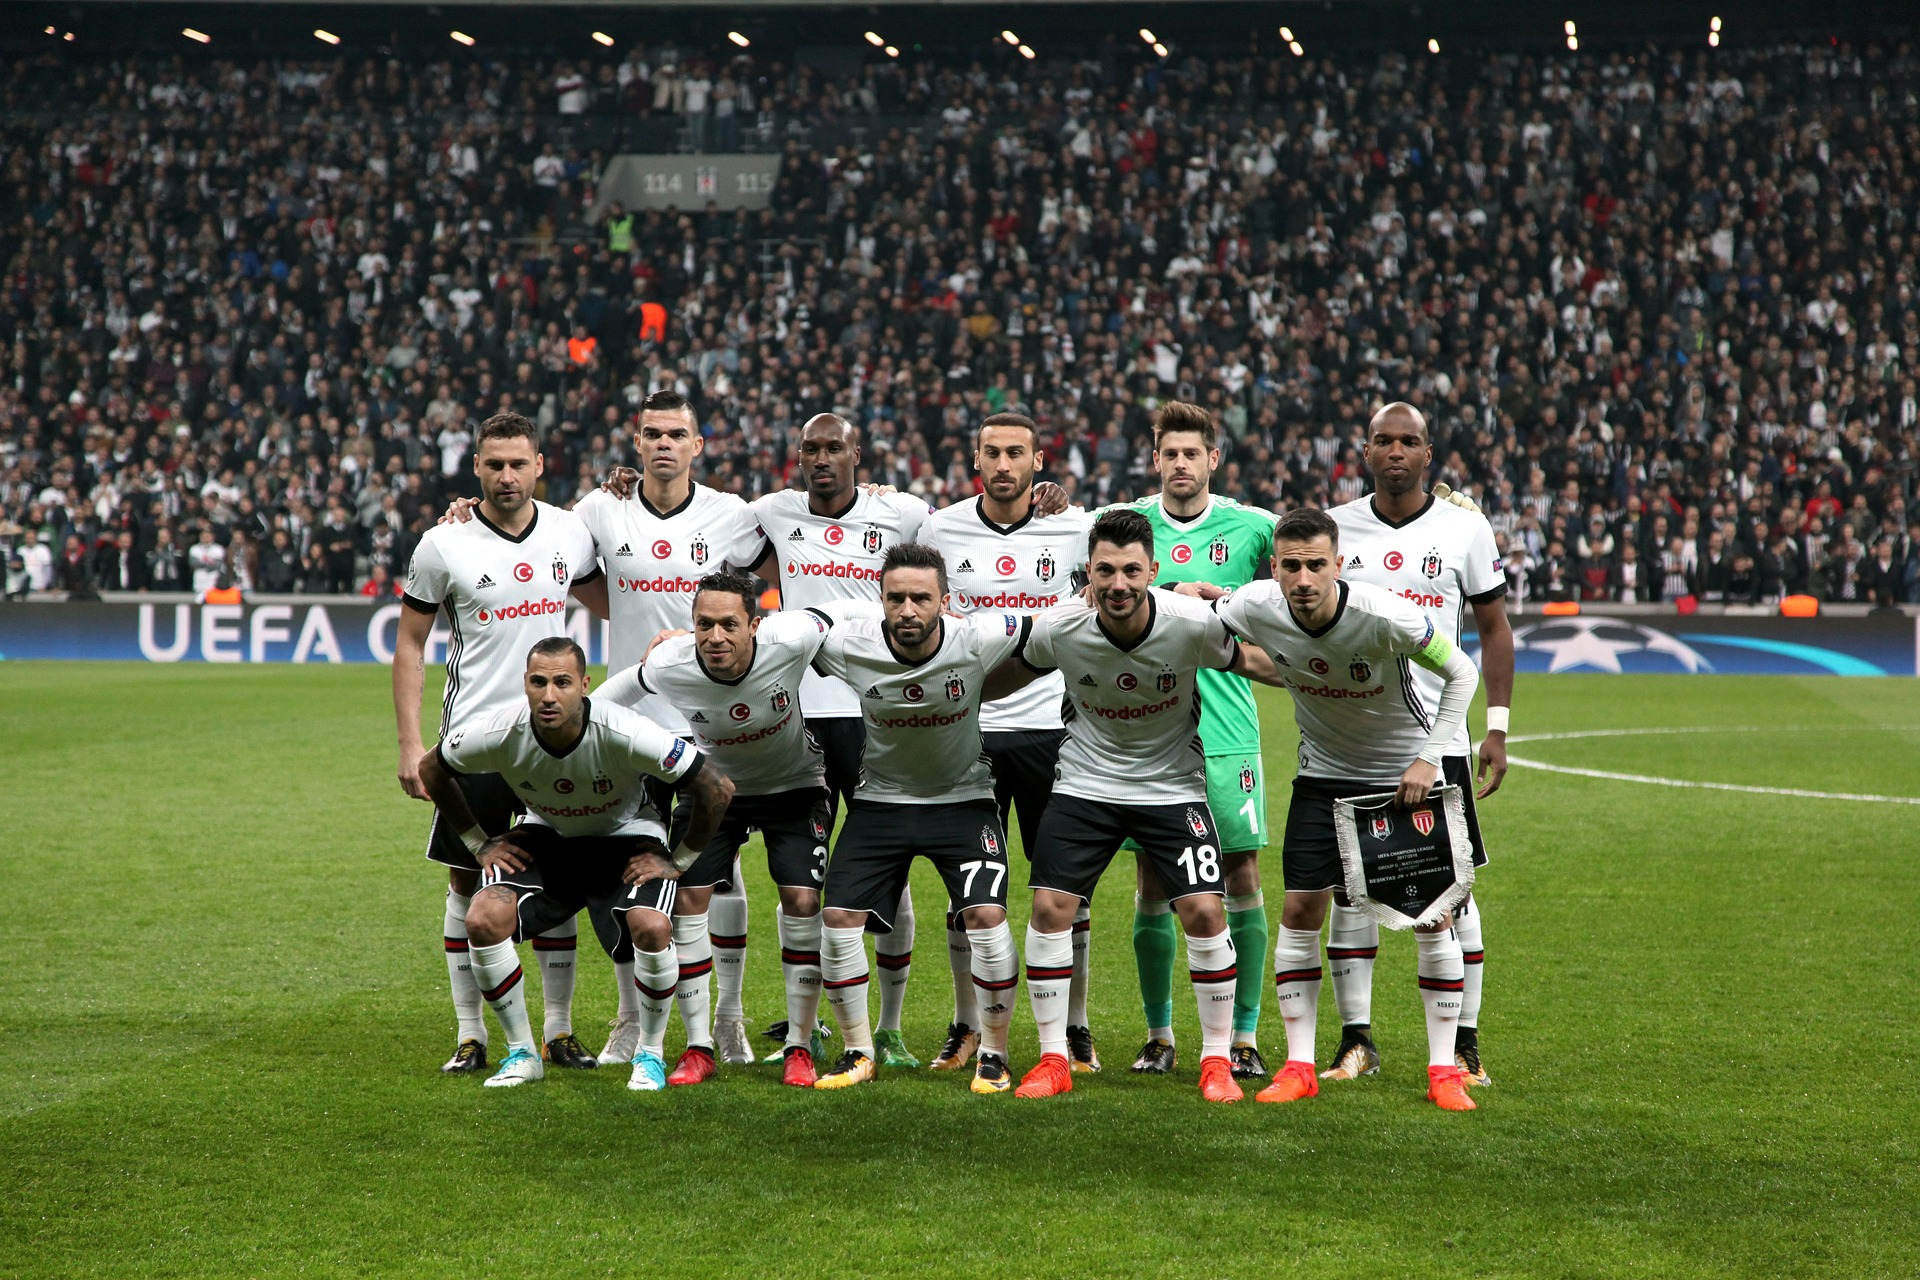
\includegraphics[width=0.75\textwidth]{besiktas_team} % sets width to 75% of textwidth
        % \caption{arg} command gives the figure a caption
        \caption{Besiktas JK 2017/2018}
        % \label{fig:<name>} command labels the figure and generates a number to reference the image within the document
        % with \ref{fig:<name>}
        % \label command have to be the last in a figure, otherwise the reference won't displayed.
        \label{fig:besiktas_team}     
    \end{figure}

    % This \includegraphics command can contain following options, comment or comment out the options you want
    % to try out.
    \begin{figure}
        \centering
        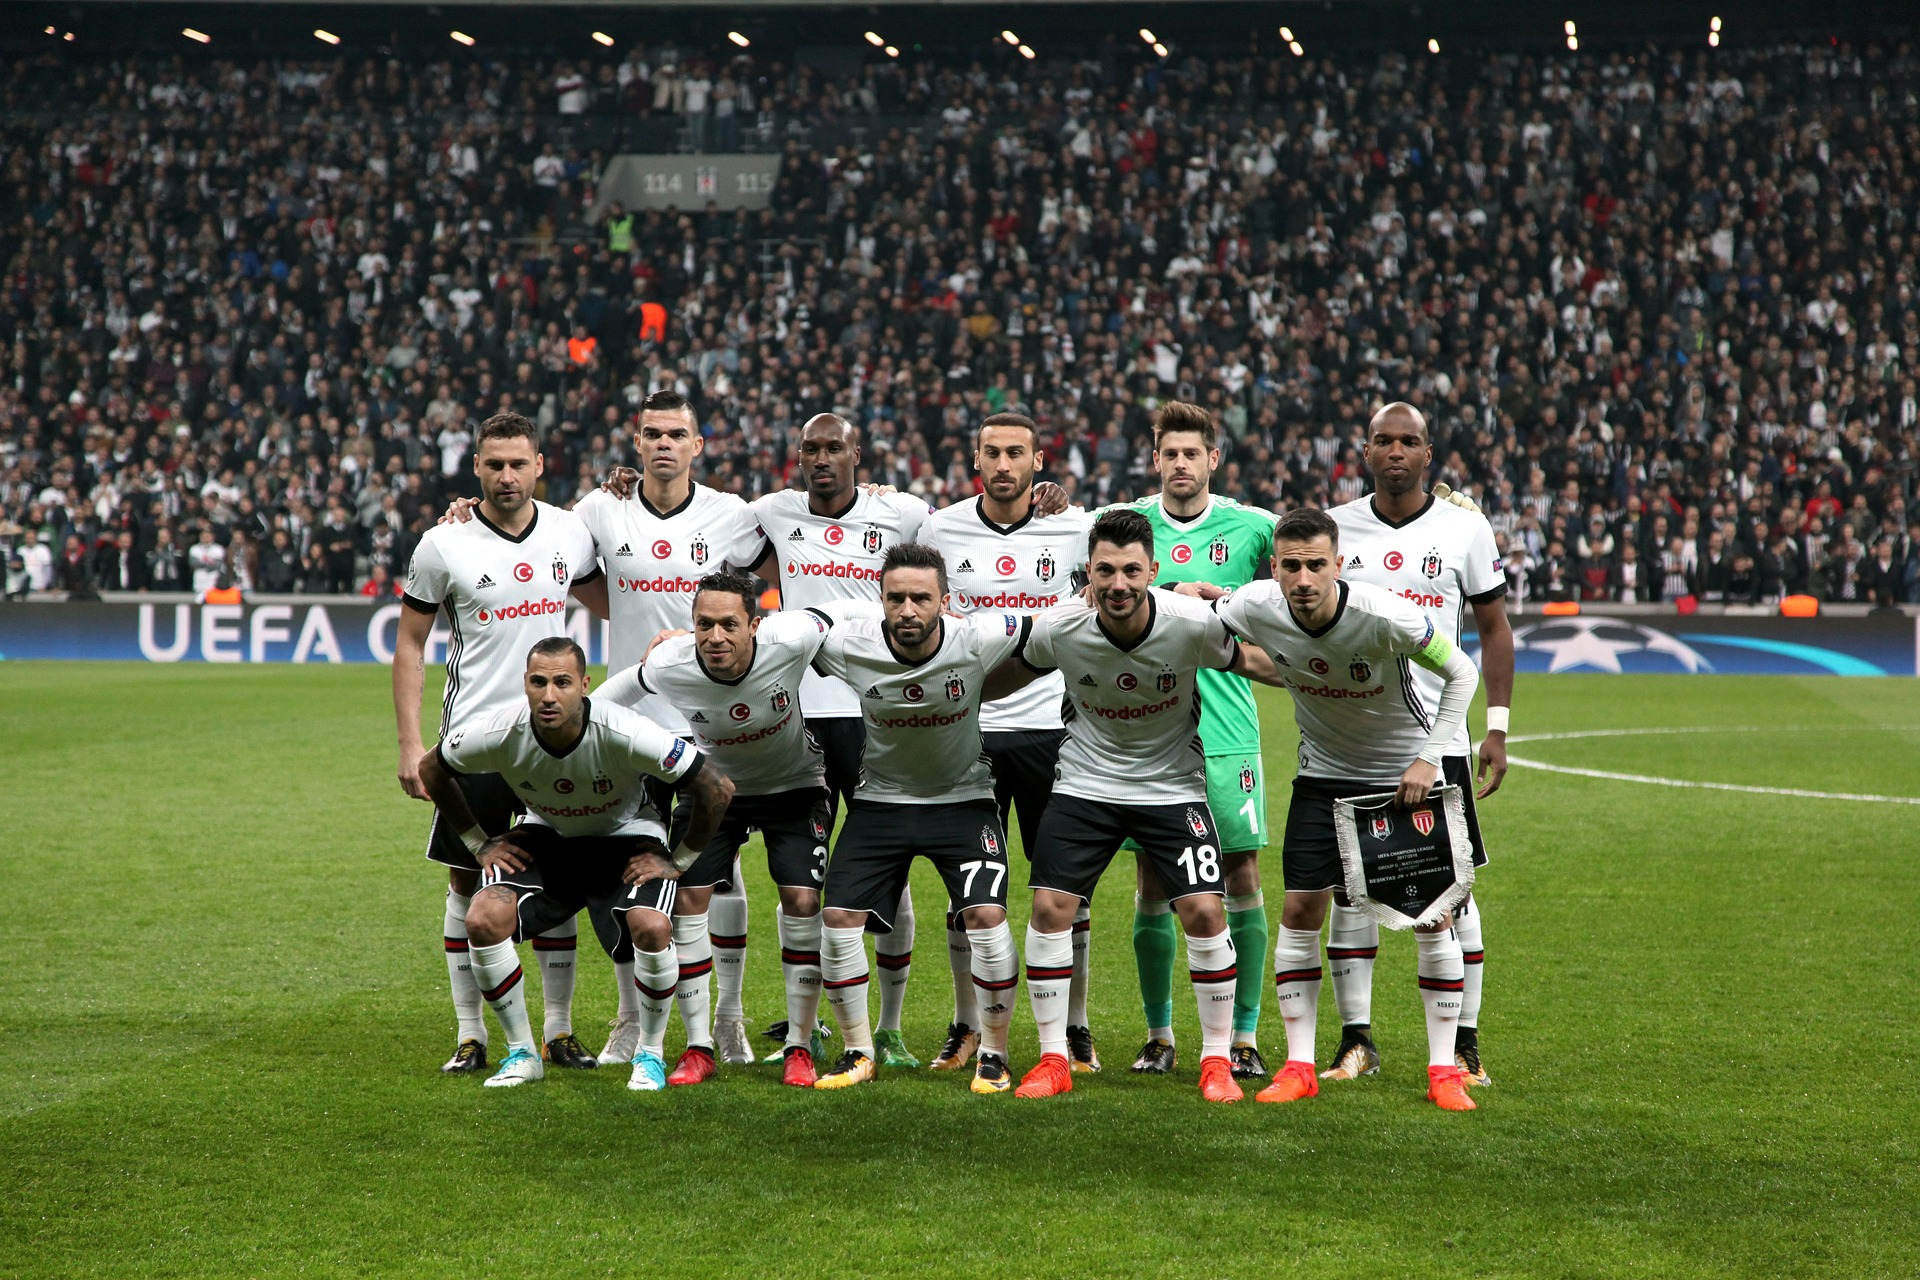
\includegraphics
        [%scale=0.10,% scale scales graphic based on specified scale factor
         %width=5.5cm,% width scales graphic based on specified width 
         height=3.5cm,% height scales graphic based on specified height
         %draft % is draft set, latex displays a placeholder (path of file) instead of loading the image. Accelerates the translation process of document.
         angle=-90,% angle rotate the graphic based on specified value, positiv values = counterclockwise, negative values = clockwise,
         % -90 rotates the graphics 90 degree clockwise
        ]{besiktas_team}
        \caption{height 3.5cm and rotate -90 degree (clockwise)}
        \label{fig:besiktas_team_with_several_options}
    \end{figure}

    % \ref{figure} command is substituted by the number corresponding to the referenced figure 
    % \pageref{figure} command is substituted by the page number on which the figure is displayed.  
    The Figure \ref{fig:besiktas_team} is on page \pageref{fig:besiktas_team}.

\end{document}


%-----------------------------------------------------------------------------------------------------------
% Sources:
%           https://www.overleaf.com/learn/latex/Learn_LaTeX_in_30_minutes#The_preamble_of_a_document
%           
%           
%           
%           
%           
%           
%           
%           
%           https://pixabay.com/photos/besiktas-sho-champions-league-2910497/ (picture: besiktas_team)
%           https://pixabay.com/photos/soccer-europe-uefa-champions-league-2698966/ (picture besiktas_flag)
% 
%
%
% 
%
%
% 
%
%
% 
%
%
% 
%
%
% 
%
%
% 
%-----------------------------------------------------------------------------------------------------------
